
The goal of this study is to answer the question, `Within five equivalence classes, what representations are more comprehensible?' by presenting programmers with one of several representations of semantically equivalent regexes and asking comprehension questions. By comparing the understandability of semantically equivalent regexes that have different representations, it is possible to infer which representations are more desirable.
This study was implemented on Amazon's Mechanical Turk with 180 participants.  Each regex was evaluated by 30 participants.
The regexes used were designed to belong to various nodes of the equivalence class graphs depicted in Figure~\ref{fig:refactoringTree}.

\begin{table}
\caption{Matching metric example \label{matchingmetric}}
\begin{center}
\begin{small}
\begin{tabular} {cl | c c c c c}
\textbf{String} & \verb!`RR*'! & \textbf{Oracle} & \textbf{P1} & \textbf{P2} & \textbf{P3}& \textbf{P4}\\ \hline
1 & ``ARROW"    & \checkmark    & \checkmark    & \checkmark    & \checkmark    & \checkmark \\
2 & ``qRs"      & \checkmark    & \checkmark    & \xmark        & \xmark        & ?\\
3 & ``R0R"      & \checkmark    & \checkmark    & \checkmark    & ?             & -\\
4 & ``qrs"      & \xmark        & \checkmark    & \xmark        & \checkmark    & -\\
5 & ``98"       & \xmark        & \xmark        & \xmark        & \xmark        & -\\
\hline
  & Score       & 1.00          & 0.80          & 0.80          & 0.50          & 1.00\\
\\
\multicolumn{7}{l}{\checkmark = match, \xmark = not a match, ? = unsure, -- = left blank}\\
\end{tabular}
\end{small}
\end{center}
\end{table}


\subsection{Metrics}
\label{sec:understandabilityMetrics}
The understandability of regexes was measured using two complementary metrics, \emph{matching} and \emph{composition}.

\textbf{Matching:}
Given a regex and a set of strings, a participant determines which strings will be matched by the regex. There are four possible responses for each string, \emph{matches}, \emph{not a match}, \emph{unsure}, or blank. An example from the study is shown in Figure~\ref{fig:exampleQuestion}.  The use of the term `matches' in this chapter is consistent with the meaning described in Section~\ref{sec:matchingDefined} - if any substring of a target string belongs to the set of strings specified by a particular regex, then that regex is said to \emph{match} that target string.


\begin{figure}[tb]
\centering
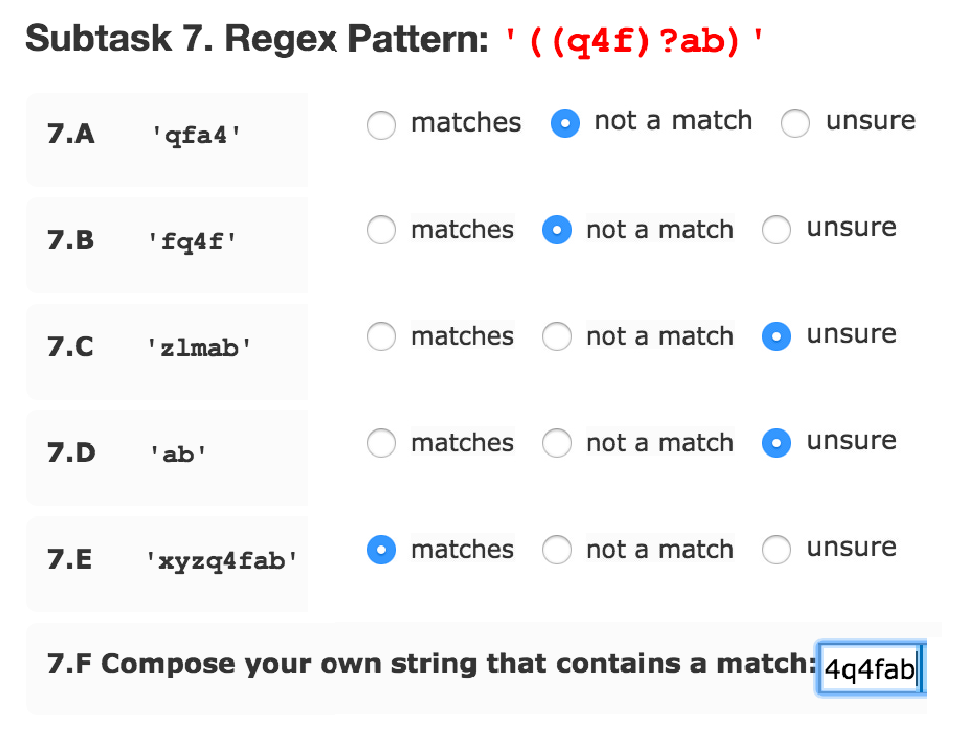
\includegraphics[width=0.54\columnwidth]{nontex/illustrations/exampleQuestion.eps}
\vspace{-12pt}
\caption{Example of one HIT Question}
\vspace{-6pt}
\label{fig:exampleQuestion}
\end{figure}

The percentage of correct responses, disregarding blanks and unsure responses, is the matching score.
For example, consider regex \cverb!RR*! and five strings shown in Table~\ref{matchingmetric}, and the responses from four participants in the \emph{P1}, \emph{P2}, \emph{P3} and \emph{P4} columns.
The oracle has the first three strings matching since they each contain at least one \verb!`R'! character. \emph{P1} answers correctly for the first three strings but incorrectly thinks the fourth string matches, so the matching score is $4/5 = 0.80$. \emph{P2} incorrectly thinks that the second string is not a match, so they also score $4/5 = 0.80$.  \emph{P3} marks `unsure' for the third string and so the total number of attempted matching questions is 4 instead of 5. \emph{P3} is incorrect about the second and fourth string, so they score $2/4 = 0.50$.  For \emph{P4}, we only have data for the first and second strings, since the other three are blank.  \emph{P4} marks `unsure' for the second matching question so only one matching question has been attempted, and it was answered correctly so the matching score is $1/1 = 1.00$.

Blanks were incorporated into the metric because questions were occasionally left blank in the study. Unsure responses were provided as an option so not to bias the  results when participants were honestly unsure of the answer.  These situations did not occur very frequently. Only 1.1\% of the responses were left blank and only 3.8\% of the responses were marked as unsure.  An investigation into the potential meaning of unsure results is in Appendix~\ref{app:unsureResults}.  A matching problem with all blank or unsure responses is referred to as an `NA'. Out of 1800 questions, 1.8\%(32) were NA's (never more than 4 out of 30 per regex).

\textbf{Composition:}
Given a regex, a participant composes a string they think it matches. If the participant is accurate and the string indeed is matched by the regex, then a composition score of 1 is assigned, otherwise 0.  For example, given the regex \cverb!(q4fab|ab)! from the study, the string \verb!"xyzq4fab"! matches and would get a score of 1, and the string \verb!"fac"! is not matched and would get a score of 0.

To determine a match, each regex was compiled using the \emph{java.util.regex} library. A
\\*\emph{java.util.regex.Matcher} {\tt m} object was created for each composed string using the compiled regex.  If {\tt m.find()} returned true, then that composed string was given a score of 1, otherwise it was given a score of 0.

\subsection{Implementation}
This study was implemented on Amazon's Mechanical Turk (MTurk),  a crowdsourcing platform in which requesters can create human intelligence tasks (HITs) for completion by workers. Each HIT is designed to be completed in a fixed amount of time and workers are compensated with money if their work is satisfactory. The IRB approval for this work is in Appendix~\ref{app:IRBMT}.  Requesters can screen workers by requiring each to complete a qualification test prior to completing any HITs.

\paragraph{Worker Qualification.} Workers qualified to participate in the study by answering questions regarding some basics of regex knowledge. These questions were multiple-choice and asked the worker to describe what the following regexes mean: \cverb!a+!, \cverb!(r|z)!, \cverb!\d!, \cverb!q*!, and \cverb![p-s]!. To pass the qualification, workers had to answer four of the five questions correctly.  The qualification is available in Appendix~\ref{app:MTqualifyingTest}.

\paragraph{Selecting pairwise comparisons.}  Using the regexes in the corpus as a guide, ten metagroups were created for this study.  The first six metagroups (re-numbered for simplicity) each contain three pairs of regexes.  The last four metagroups contain two sets of three equivalent regexes.  A list of the specific regexes selected for these metagroups is available in Appendix~\ref{app:MTstudyInput}.

\begin{multicols}{2}
\begin{description}[noitemsep,topsep=0pt]
\item[M1]  S1 vs S2
\item[M2]  C1 vs C4, focusing on DEC
\item[M3]  C1 vs C4, focusing on WRD
\item[M4]  C4 vs (C3 or C2)
\item[M5]  L2 vs L3
\item[M6]  T1 vs T3
\item[M7]  D1 vs D2 vs D3
\item[M8]  C1 vs C2 vs C5
\item[M9]  C2/T1 vs C5/T1 vs C2/T4
\item[M10] C1/T2 vs C1/T4 vs C2/T1
\end{description}
\end{multicols}

Each of these 10 metagroups contains 6 regexes, resulting in a total of 60 regexes.  These regexes are logically partitioned into 26 semantic equivalence groups (18 from pairs, 8 from triples).

Although this design provides 42 pairwise comparisons (18 from pairs, 24 from triples),  seven total comparisons had to be dropped due to design flaws.  For six of the comparisons, the regexes performed transformations from multiple equivalence classes, making it impossible to tell which edge to attribute the results to. For example \\*\cverb!([\072\073])! is in C2 and T4.  This regex was paired with \cverb!(:|;)! in C5, T1, so it was not possible to attribute results purely to C2 and C5, or to T4 and T1. However, the third member of the group, \cverb!([:;])!, could be compared with both, since it is a member of T1 and C2, so comparing it to \cverb!([\072\073])! evaluates the transformation between T1 and T4, and comparing to \cverb!(:|;)! evaluates the transformation between C2 and C5.  The seventh pair: \cverb!\..*! and \cverb!\.+! between L2 and L3, had to be dropped because these two regexes are not equivalent.  The first regex was meant to be \cverb!\.\.*!.  Data gathered for all seven of these flawed pairings was ignored.

An example of a correct pairwise comparison from a pair used in this study is a group with regexes \cverb!([0-9]+)\.([0-9]+)! and  \cverb!(\d+)\.(\d+)!, which is intended to evaluate the edge between C1 and C4.
An example of pairwise comparisons from a triple is a semantic group with regexes \cverb!((q4f){0,1}ab)!, \cverb!((q4f)?ab)!, and \cverb!(q4fab|ab)! which is intended to explore the edges among D1, D2, and D3.

The end result is 35 pairwise comparisons across 14 edges from Figure~\ref{fig:refactoringTree}.

\paragraph{Composing Tasks.}  For each of the 26 groups of regexes, five strings were created, where at least one matched and at least one did not match. These strings were used to compute the matching metric. A list of the specific strings created is available in Appendix~\ref{app:MTstudyInput}.

Once all the regexes and matching strings were collected, tasks for the MTurk participants were created as follows: randomly select a regex from each of the 10 metagroups. Randomize the order of these 10 regexes, as well as the order of the matching strings for each regex. The randomly selected regexes and shuffled matchings strings populate fields in an HTML template (Appendix~\ref{app:MTtemplate}).  This template also includes a request for participants to compose a string that matches each of the 10 regexes.  Each populated template created one HIT.
This process was completed until each of the 60 regexes appeared in 30 HITs, resulting in a total of 180 total unique HITs.
% An example of a single regex, the five matching strings and the space for composing a string is shown in Figure~\ref{fig:exampleQuestion}.

\paragraph{Worker statistics.}\label{sec:workerStatistics} Workers were paid \$3.00 for successfully completing a HIT, and were only allowed to complete  one HIT.  The average completion time for accepted HITs was 682 seconds (11 mins, 22 secs).
A total of 55 HITs were rejected, and  of those, 48 were rushed through by one person leaving many answers blank, 4 other HITs were also rejected because a worker had submitted more than one HIT.  All worker composition answers were inspected to make sure that the composition answer was composed in a good-faith effort to  match the regex before accepting the HIT (the field was not empty, and the content seemed like it had required some thought). One worker was rejected for not answering composition sections, and one was rejected because it was missing data for 3 questions.  Rejected HITs were returned to MTurk to be completed by others.
